\documentclass[12pt]{article}

\usepackage{fancyhdr}
\usepackage{extramarks}
\usepackage{amsmath} %\usepackage{amsthm}
\usepackage{amsfonts}
\usepackage{tikz}
%\usepackage{gensymb}
%\usepackage[plain]{algorithm}
\usepackage{cancel}
%\usepackage{algpseudocode}
%\usepackage{mathtools}
\usepackage{empheq}
\usepackage{siunitx}
\usepackage{bm}
\usepackage{physics}

\usetikzlibrary{automata,positioning}
\usetikzlibrary{arrows.meta}

%
% Basic Document Settings
%

\topmargin=-0.45in
\evensidemargin=0in
\oddsidemargin=0in
\textwidth=6.5in
\textheight=9.0in
\headsep=0.25in

\linespread{1.1}

\pagestyle{fancy}
\lhead{\hmwkAuthorName}
\chead{\hmwkClass\ (\hmwkClassInstructor): \hmwkTitle}
\rhead{\firstxmark}
\lfoot{\lastxmark}
\cfoot{\thepage}

\renewcommand\headrulewidth{0.4pt}
\renewcommand\footrulewidth{0.4pt}

\DeclareMathOperator{\arccosh}{arccosh}

\setlength\parindent{0pt}

%
% Create Problem Sections
%

\newcommand{\enterProblemHeader}[1]{
	\rhead{#1}
}

\newcommand{\exitProblemHeader}[1]{
	\pagebreak
}

%
% Homework Problem Environment
%
% This environment takes an optional argument. When given, it will adjust the
% problem counter. This is useful for when the problems given for your
% assignment aren't sequential. See the last 3 problems of this template for an
% example.
%
\newenvironment{homeworkProblem}[1]{
    \section{Problem #1}
    \enterProblemHeader{#1}
}{
	\pagebreak
}

\newenvironment{main_section}[1]{
	\section{#1}
	\enterProblemHeader{#1}
}{
	\pagebreak
}

%
% Homework Details
%   - Title
%   - Due date
%   - Class
%   - Section/Time
%   - Instructor
%   - Author
%

\newcommand{\hmwkTitle}{Project}
\newcommand{\hmwkDueDate}{April 29, 2020}
\newcommand{\hmwkClass}{Waves \& Optics}
\newcommand{\hmwkClassInstructor}{Prof. Peifen Zhu}
\newcommand{\hmwkAuthorName}{\textbf{Joseph Mellor}}

%
% Title Page
%

\title{
    \vspace{2in}
    \textmd{\textbf{\hmwkClass:\ \hmwkTitle}}\\
    \normalsize\vspace{0.1in}\small{Due\ on\ \hmwkDueDate}\\
    \vspace{0.1in}\large{\textit{\hmwkClassInstructor}}
    \vspace{3in}
}

\author{\hmwkAuthorName}
\date{}

%
% Various Helper Commands
%

% Useful for algorithms
\newcommand{\alg}[1]{\textsc{\bfseries \footnotesize #1}}

% For derivatives
\newcommand{\deriv}[2]{\frac{d#1}{d#2}}

% For partial derivatives
\newcommand{\pderiv}[2]{\frac{\partial #1}{\partial #2}}

% Integral dx
\newcommand{\dx}[1]{\mathrm{d}#1}

% Alias for the Solution section header
\newcommand{\solution}{\textbf{\large Solution}}

% Probability commands: Expectation, Variance, Covariance, Bias
\newcommand{\E}{\mathrm{E}}
\newcommand{\Var}{\mathrm{Var}}
\newcommand{\Cov}{\mathrm{Cov}}
\newcommand{\Bias}{\mathrm{Bias}}

\newcommand{\R}{\mathbb{R}}
\newcommand{\Z}{\mathbb{Z}}
\newcommand{\Q}{\mathbb{Q}}
\newcommand{\N}{\mathbb{N}}
\newcommand{\C}{\mathbb{C}}

\newcommand{\tensor}[1]{\overset{\leftrightarrow}{#1}}

\newcommand\ddfrac[2]{\frac{\displaystyle #1}{\displaystyle #2}}
\DeclarePairedDelimiter\ceil{\lceil}{\rceil}
\DeclarePairedDelimiter\floor{\lfloor}{\rfloor}

\begin{document}

\maketitle

\pagebreak

\begin{main_section}{Goal}
	In order to maximize the light extraction efficiency, we must maximize the
	total amount of light transmitted from the point source through the top of
	the LED. The light escaping through the sides will be negligible.

	\subsection{Model}

	We are going to model the LED as a point source in a medium of constant
	refractive index, with one side reflecting all light that hits it and the
	other side reflecting and transmitting the light based on the physical
	properties at the boundary. We can model reflections as having a virtual
	point source on the opposite side of the mirror with the materials also
	being mirrored, and we will use this model to make our calculations simpler.
	Lastly, we will model the entire LED as one medium since it has the same
	exact index of refraction throughout it. We will use the symbols $d$ to
	represent the entire thickness of the LED and $d_0$ to represent the
	distance from the Air-LED Boundary.

	\definecolor{crimson}{HTML}{DC143C}
	\definecolor{cool-crimson}{HTML}{B91161}
	\definecolor{mid-red}{HTML}{F31AA0}
	\definecolor{cool-pink}{HTML}{E30BE1}
	\definecolor{cool-violet}{HTML}{A109D0}
	\definecolor{air}{HTML}{D5D4FF}
	\definecolor{light-brown}{HTML}{E0E284}
	\definecolor{light-green}{HTML}{F7F79C}
	\definecolor{silver}{HTML}{C0C0C0}

	\begin{figure}[h]
	\centering
	\begin{tikzpicture}[scale=1.3]
		\fill[air] (-4, 1) rectangle (4, 3);
		\fill[air] (-4, 3) -- (-3, 4) -- (5, 4) -- (4, 3);
		\fill[air] (5, 4) -- (4, 3) -- (4, 1) -- (5, 2);
		\fill[light-green] (-4, -3) rectangle (4, 1);
		\fill[light-green] (-4, 1) -- (4, 1) -- (5, 2) -- (-3, 2);
		\fill[light-green] (4, -3) -- (5, -2) -- (5, 2) -- (4, 1);
		\fill[silver] (-4, -1) -- (-3, 0) -- (5, 0) -- (4, -1);
		\foreach \a in {-2, 0, 2}
			\draw[dashed] (-3, \a) -- (5, \a);
		\foreach \d in {0.2, 0.5, 0.8}
			\foreach \b/\c in {-2/cool-violet, 0/cool-crimson}
				\foreach \a in {-3,-1.5,...,3}
					\draw[\c,line width=0.4mm,dotted,-{Latex[length=3mm]}] (0 + 0.5, \b + 0.5) -- (\a + \d, 1
					+ \d);
		\draw (4, 1) -- (-4, 1) node [anchor=east, inner sep = 20pt] {Air-LED Boundary};
		\draw[cool-crimson,fill=cool-crimson] (0.5, 0.5) circle (0.12);
		\node[draw,fill=white] at (0.5, 0)
		{{\boldmath$\color{cool-crimson}{P_0}$}};
		\draw (4, -1) -- (-4, -1) node [anchor=east, inner sep = 20pt] {Silver Reflector};
		\draw[cool-violet,fill=cool-violet] (0.5, -1.5) circle (0.12);
		\node[draw,fill=white] at (0.5, -2)
		{{\boldmath$\color{cool-violet}{P_1}$}};
		\foreach \a in {-3,-1,1}
			\foreach \b/\c in {-4/dashed, 4/}
				\draw[\c] (\b, \a) -- (\b + 1, \a + 1);
		\draw[dashed] (-3, -2) -- (-3, 2);
		\draw (-4, -3) rectangle (4, 1);
		\draw (5, -2) -- (5, 2);
		\draw[|<->|,line width=0.3mm] (-4.2, -1) -- (-4.2, 0) node[midway, left]
		{$d - d_0$};
		\draw[|<->|,line width=0.3mm] (-4.2, 0) -- (-4.2, 1) node[midway, left]
		{$d_0$};
		\draw[|<->|,line width=0.3mm] (-4.2, -2) -- (-4.2, -3) node[midway,
		left] {$d_0$};
		\draw[|<->|,line width=0.3mm] (-4.2, -2) -- (-4.2, -1) node[midway,
		left] {$d - d_0$};
	\end{tikzpicture}
	\caption{Our Model}
	\end{figure}

	The light at $P_0$ and $P_1$ should produce the exact same amount of light.

	\subsection{Higher Order Model}

	There will also be virtual point sources below $P_1$ because the light
	reflected at the Air-LED Boundary will then bounce off the silver reflector,
	some of which will bounce off the Air-LED Boundary, which will then bounce
	off the silver and so on. It will be an infinite sum of virtual point
	sources with less light as they get farther from the Air-LED Boundary. The
	distance away from the Air-LED Boundary for the $n^\text{th}$ will be
	\[
		d_n =
		\begin{cases}
		d_0 + nd, & n\quad\text{even}\\
		d - d_0 + nd, & n\quad\text{odd}
		\end{cases}
	\]
	Furthermore, the intensity of light for the $n^\text{th}$ point source will
	be
	\begin{align*}
		I_n(\theta_I, r) = P_0 \left(R(\theta_I)\right)^{\lfloor n / 2 \rfloor}
		r^{-2}
	\end{align*}
	where $R$ is the $i^\text{th}$ reflection coefficient for a given
	$\theta_I$ and $r$ is the distance from the point because intensity follows
	an inverse square law.
\end{main_section}

\begin{main_section}{Initial Efficiency}
	In this section, I will calculate the efficiency of the LED as presented in
	the model.
	\begin{align*}
		\theta_I &= \arctan \left( \frac \rho {d_n} \right)\\
		&= \arcsin \left( \frac \rho {\sqrt{\rho^2 + d_n^2}} \right)\\
		&= \arccos \left( \frac {d_n} {\sqrt{\rho^2 + d_n^2}} \right)\\
	\end{align*}
	We'll need Eqs. (9.110), (9.106), (9.116), and (9.200) to get $\alpha$,
	$\beta$, $R$ (reflection coefficient), $T$ (transmission coefficient), and
	$\theta_C$ (the critical angle).
	\begin{align*}
		\alpha &= \frac { \sqrt{1 - \beta^{-2} \sin^2 \theta_I} } {\cos \theta_I}
		\tag{9.110}\\
		\beta &= \frac {\mu_1 n_2} {\mu_2 n_1} \approx 0.4 \tag{9.106}\\
		R &= \left( \frac { \alpha - \beta } { \alpha + \beta } \right)^2
		\tag{9.115}\\
		T &= \alpha \beta \left( \frac 2 {\alpha + \beta} \right)^2\tag{9.116}\\
		\theta_C &= \arcsin \beta \tag{9.200} \approx 23.578^\circ
	\end{align*}
	where we made the simplification $\mu_1 = \mu_2$.

	\subsection{Using the Critical Angle}

	Any light outside of the critcal angle will be internally reflected, so we
	can ignore it, meaning our integration region will be smaller for lower
	order point sources (and possibly circular). Since $d_n$ increases
	approximately linearly, we can find an upper bound on $n$ where our
	integration region is a circle by considering $n d \tan \theta_C =
	x_\text{max}$. We can also use $d < 10 \si{\mu m}$ to get a hard upper
	bound.
	\begin{align*}
		n (10 \si{\mu m}) \tan(23.578^\circ) &< 300 \si{\mu m}\\
		n < \frac {30} {\tan(23.578^\circ)}\\
		n < 68.7\\
		n < 69 % Nice
	\end{align*}
	So for 68 internal reflections, all the light that can pass through will be
	within a circle of radius $d_n \tan \theta_C$.

	\subsection{Infinitesimal Transmission}

	Let $L$ be the amount of light passing through the Air-LED Boundary and $dL$
	be the differential amount of light passing through some $dA$ for a given
	$(x, y)$ or $\theta_I \in [0, \theta_C)$.
	\begin{align*}
		dL &= I_n(\theta_I) \frac T {x^2 + y^2 + d_n^2} dx dy\\
		&= P_0 (1 - T)^{\lfloor n / 2 \rfloor} \frac T {x^2 + y^2 + d_n^2} dx
		dy\\
		&= P_0 (1 - T)^{\lfloor n / 2 \rfloor} \frac T {d_n^2 \sec^2 \theta_I}
		(2 \pi \tan \theta_I) d \theta\\
		&= \frac {\pi P_0} {d_n^2} (1 - T)^{\lfloor n / 2 \rfloor} T \sin (2
		\theta_I) d \theta
	\end{align*}

	\subsection{Total Efficiency}

	The total amount of light passing through the surface of the LED from the
	$n^\text{th}$ order term is therefore
	\begin{align*}
		L(n) &= \int dL\\
		&= \frac {2 \pi P_0} {d_n^2} \int_0^{\theta_C} R^{\lfloor n / 2 \rfloor}
		(1 - R) \sin \theta_I \cos \theta_I d\theta_I\\
		&= \frac {2 \pi P_0} {d_n^2} \int_0^{\theta_C} \sin \theta_I \cos
		\theta_I \left( R^N - R^{N + 1} \right) d\theta_I\\
		&= \frac {2 \pi P_0} {d_n^2} \left( \int_0^{\theta_C} R^N \sin \theta_I
		\cos \theta_I d\theta_I - \int_0^{\theta_C} R^{N + 1} \sin \theta_I \cos
		\theta_I d\theta_I \right)\\
		&= \frac {2 \pi P_0} {d_n^2} \left( \zeta(N, \beta) - \zeta(N + 1,
		\beta) \right)
	\end{align*}
	where $N = \lfloor n / 2 \rfloor$, but I'm currently treating it as if it's
	independent of $n$ to make the math easier. Also, I defined the new function
	\begin{align*}
		\zeta(\mathcal N, \beta) &= \int_0^{\theta_C} R^{\mathcal N} \sin
		\theta_I \cos \theta_I d\theta_I\\
		&= \int_0^{\theta_C} \left( \frac {\alpha - \beta} {\alpha + \beta}
		\right)^{2 \mathcal N} \sin \theta_I \cos \theta_I d\theta_I\\
		&= \int_0^{\theta_C} \left( \frac {\frac {\sqrt{1 - \beta^{-2}\sin^2
		\theta_I} } {\cos \theta_I } - \beta} {\frac {\sqrt{1 - \beta^{-2}\sin^2
		\theta_I} } {\cos \theta_I } + \beta} \right)^{2 \mathcal N} \sin
		\theta_I \cos \theta_I d\theta_I\\
		&= \int_0^{\theta_C} \left( \frac { \sqrt{1 - \beta^{-2} \sin^2
		\theta_I} - \beta \cos \theta_I } { \sqrt{1 - \beta^{-2} \sin^2
		\theta_I} + \beta \cos \theta_I } \right)^{2 \mathcal N} \sin \theta_I
		\cos \theta_I d \theta_I
	\end{align*}
	Letting $u = \beta^{-1} \sin \theta_I$ means $\beta du = \cos \theta_I d
	\theta_I$ and $\cos \theta_I = \sqrt{ 1 - \beta^2 u^2 }$, so
	\begin{align*}
		\zeta( \mathcal N, \beta ) &= \int_0^1 \left( \frac { \sqrt{ 1 - u^2 } -
		\beta \sqrt{ 1 - \beta^2 u^2 } } { \sqrt{ 1 - u^2 } + \beta \sqrt{ 1 -
		\beta^2 u^2 } } \right)^{2 \mathcal N} \beta u \beta du\\
		&= \beta^2 \int_0^1 u \left( \frac { \sqrt{1 - u^2} - \beta \sqrt{1 -
		\beta^2 u^2} } { \sqrt{1 - u^2} + \beta \sqrt{1 - \beta^2 u^2}
		}\right)^{2 \mathcal N} du\\
		&= \beta^2 \int_0^1 u \left( 1 - \frac {2 \beta \sqrt{1 - \beta^2 u^2} }
		{ \sqrt{ 1 - u^2 } + \beta \sqrt{ 1 - \beta^2 u^2 } } \right)^{2
		\mathcal N} du
	\end{align*}
	Using the binomial theorem, we find
	\begin{align*}
		\zeta( \mathcal N, \beta ) &= \beta^2 \int_0^1 u \sum_{k = 0}^{2
		\mathcal N} \binom {2 \mathcal N} k \left( - \frac {2 \beta \sqrt{ 1 -
		\beta^2 u^2 } } { \sqrt{1 - u^2} + \beta \sqrt{ 1 - \beta^2 u^2 } }
		\right)^k du
	\end{align*}
	Letting $v = u^2$ and interchanging the sum and the integral (since there
	are only a finite number of well-behaved terms) yields
	\begin{align*}
		\zeta(\mathcal N, \beta) &= \frac 12 \beta^2 \sum_{k = 0}^{2 \mathcal N}
		\binom {2 \mathcal N} k \int_0^1 \left( - \frac { 2 \beta \sqrt{1 -
		\beta^2 v} } {\sqrt{1 - v} + \beta \sqrt{1 - \beta^2 v} } \right)^k dv\\
		&= \frac 12 \beta^2 \sum_{k = 0}^{2 \mathcal N} \binom {2 \mathcal N} k
		\eta(\beta, k)\\
		\eta(\beta, k) &= \int_0^1 \left( - \frac { 2 \beta \sqrt{1 -
		\beta^2 v} } {\sqrt{1 - v} + \beta \sqrt{1 - \beta^2 v} } \right)^k dv
	\end{align*}
	At this point, the integral probably can't be solved analytically (except in
	the trivial case where $k = 0$), but it can be easily evaluated with
	numerical methods, I'm just going to have a table for all the relevant
	values of $\eta(\beta, k)$ and $\zeta(\mathcal N, \beta)$ in this project in
	an appendix. I wrote my own C++ program to evaluate this integral, and since
	I have yet to use a higher precision than IEEE-754 quad, these figures are
	at most guaranteed to be accurate to six significant figures.
\end{main_section}

\begin{main_section}{Appendix}
	\subsection{Values of $\eta (0.4, k)$}
	\begin{center}
	\begin{tabular}{r|r|r|r|r}
		 k    &   $\eta(0.4, k)$      &   &   k   & $\eta(0.4, k)$\\
		 \hline
		 0    &    1.000000000000000  &   &  21   &   -1484.95318419670\\
		 1    &   -0.778582843102452  &   &  22   &    2686.77263734128\\
		 2    &    0.653960057739195  &   &  23   &   -4884.60026011296\\
		 3    &   -0.602415444402244  &   &  24   &    8919.01516065738\\
		 4    &    0.615052623011061  &   &  25   &   -16350.4364164837\\
		 5    &   -0.696155362847541  &   &  26   &    30083.0576002128\\
		 6    &    0.864909739583435  &   &  27   &   -55535.1340978725\\
		 7    &   -1.161195899155380  &   &  28   &    102838.249544306\\
		 8    &    1.657417436796580  &   &  29   &   -190977.779844026\\
		 9    &   -2.480312863079820  &   &  30   &    355601.318988541\\
		10    &    3.850083438680390  &   &  31   &   -663768.336987781\\
		11    &   -6.150203762867390  &   &  32   &    1241854.27727547\\
		12    &    10.05218329304340  &   &  33   &   -2328417.93879907\\
		13    &   -16.73940170062670  &   &  34   &    4374503.58238136\\
		14    &    28.31047646171000  &   &  35   &   -8234189.43321216\\
		15    &   -48.50936611241630  &   &  36   &    15527036.8273256\\
		16    &    84.05241365620700  &   &  37   &   -29328344.8304169\\
		17    &   -147.0498739908860  &   &  38   &    55485188.6865727\\
		18    &    259.4408023090280  &   &  39   &   -105128321.877979\\
		19    &   -461.1430442674530  &   &  40   &    199471620.423876\\
		20    &    825.0781779295780  &   &       &
	\end{tabular}
	\end{center}
	\subsection{Tables of $\zeta(\mathcal N, \beta)$}
	\begin{center}
	\begin{tabular}{r|l}
		$\mathcal N$ & $\zeta(\mathcal N, \beta)$\\
		\hline
		 0&    0.08                \\
		 1&    0.00774354972274331 \\
		 2&    0.00118558555419566 \\
		 3&    0.000268946167394228\\
		 4&    0.000100818284305868\\
		 5&    0.0000557689052844639\\
		 6&    0.0000373290082928625\\
		 7&    0.0000272431233756686\\
		 8&    0.0000208575869800538\\
		 9&    0.0000164974590396467\\
		10&    0.0000133763837661169\\
		11&    0.0000110637262753572\\
		12&    0.00000930239679964554\\
		13&    0.00000793017349915641\\
		14&    0.00000684040849583049\\
		15&    0.0000059606264218156\\
		16&    0.00000524017911324007\\
		17&    0.00000464280969036029\\
		18&    0.00000414201235417406\\
		19&    0.00000371804783402861\\
		20&    0.00000335597231608467\\
	\end{tabular}
	\end{center}
\end{main_section}

\begin{homeworkProblem}{9.2}
	Show that the standing wave $f(z, t) = A \sin(kz) \cos(kvt)$ satisfies the
	wave equation, and express it as the sum of a wave traveling to the left and
	a wave traveling to the right (Eq. 9.6).

	\begin{equation}\tag{9.6}
		f(z, t) = g(z - vt) + h(z + vt)
	\end{equation}

	\solution

	Using the Product to Sum Identities yields:

	\begin{align*}
		A \sin(kz) \cos(kvt) &= \frac 12 A \left( \sin(kz + kvt) + \sin(kz -
		kvt) \right)\\
		&= \frac 12 A \sin(k(z + vt)) + \frac 12 A \sin(k(z - vt))\\
		&\implies g(x) = h(x) = \frac 12 A \sin(kx)\\
	\end{align*}

	Since we found a $g(x)$ and an $h(x)$ that satisfy both equation (9.6) and
	the given equation for the standing wave, we have shown that the standing
	wave $f(z, t) = A \sin(kz) \cos(kvt)$ satisfies the wave equation.
\end{homeworkProblem}

\begin{homeworkProblem}{9.9}
	Write down the (real) electric and magnetic fields for a monochromatic plane
	wave of amplitude $E_0$ , frequency $\omega$, and phase angle zero that is
	(a) traveling in the negative $x$ direction and polarized in the $z$
	direction; (b) traveling in the direction from the origin to the point (1,
	1, 1), with polarization parallel to the $xz$ plane. In each case, sketch
	the wave, and give the explicit Cartesian components of $\hat k$ and $\hat
	n$.

	\begin{align*}
		\vec E(\vec r, t) &= E_0 \cos(\vec k \cdot \vec r - \omega t + \delta)
		\hat n\tag{9.51}\\
		\vec B(\vec r, t) &= \frac 1c E_0 \cos(\vec k \cdot \vec r - \omega t +
		\delta) (\hat k \times \hat n)\tag{9.52}
	\end{align*}

	\solution

	One subsection for each part.

	\subsection{Part (a)}

	\begin{align*}
		\hat k &= - \hat x\\
		\hat n &= \hat z\\
		\vec k &= - \frac \omega c \hat x\\
		\vec E &= E_0 \cos \left( \omega \left( \frac {\hat x \cdot \vec r} c +
		t\right) \right) \hat z\\
		\vec B &= \frac 1 c \hat k \times \vec E\\
		&= \frac {E_0} c \cos \left( \omega \left( \frac {\hat x \cdot \vec r} c
		+ t \right) \right) \hat y
	\end{align*}

	\subsection{Part (b)}

	\begin{align*}
		\hat k &= \frac 1 {\sqrt{3}} \left( \hat x + \hat y + \hat z \right)\\
		\vec k &= \frac 1 {\sqrt{3}} \frac \omega c \left( \hat x + \hat y +
		\hat z \right)\\
		\hat n &= \frac {\hat y \times \left( \hat x + \hat y + \hat z \right)}
		{\left| \hat y \times \left( \hat x + \hat y + \hat z \right) \right|}\\
		&= \frac {\hat x - \hat z} {\left| \hat x - \hat z \right|}\\
		&= \frac 1 {\sqrt{2}} \left( \hat x - \hat z \right)
	\end{align*}
	where the derivation of $\hat n$ used a cross product between the normal of
	the plane (as a vector perpendicular to the normal of a plane is parallel to
	the plane) and the direction of propagation since it must also be
	perpendicular to the direction of propagation.
	\begin{align*}
		\vec E &= \frac {E_0} {\sqrt{2}} \cos \left( \omega \left( \frac {
		\left( \hat x + \hat y + \hat z \right) \cdot \vec r } {c \sqrt{3} } - t
		\right) \right) \left( \hat x - \hat z \right)\\
		\hat k \times \hat n &= \frac 1 {\sqrt{3}} \left( \hat x + \hat y + \hat
		z \right) \times \frac 1 {\sqrt{2}} \left( \hat x - \hat z \right)\\
		&= \frac 1 {\sqrt{6}} \left( - \hat x + 2 \hat y - \hat z \right)\\
		\vec B &= \frac {E_0} {c \sqrt{2}} \cos \left( \omega \left( \frac
		{(\hat x + \hat y + \hat z) \cdot \vec r} {c \sqrt{3}} - t \right)
		\right) ( \hat k \times \hat n)\\
		&= \frac 1 {2 \sqrt{3}} \frac {E_0} c \cos \left( \omega \left( \frac
		{(\hat x + \hat y + \hat z) \cdot \vec r} {c \sqrt{3}} - t \right)
		\right) (- \hat x + 2 \hat y - \hat z)
	\end{align*}

\end{homeworkProblem}

\begin{homeworkProblem}{9.10}
	The intensity of sunlight hitting the earth is about $1300 \si{W/m^2}$. If
	sunlight strikes a perfect absorber, what pressure does it exert? How about
	a perfect reflector? What fraction of atmospheric pressure does this amount
	to?\\
	\begin{align*}
		P = \frac 1 A \frac {\Delta p} {\Delta t} = \frac 12 \varepsilon_0 E_0^2
		= \frac I c \tag{9.64}
	\end{align*}

	\solution

	\subsection{Perfect Absorber}
	\[
		P = \frac {1300 \si{W/m^2} } {3 \times 10^8 \si{m/s} } \approx 4.336
		\times 10^{-6} \si{Pa}
	\]
	\subsection{Perfect Reflector}

	It's just twice the value for the perfect absorber, so
	\[
		P \approx 2 \times 4.336 \times 10^{-6} \si{Pa} \approx 8.673 \times
		10^{-6} \si{Pa}
	\]
	\subsection{Comparison to Atmospheric Pressure}

	\[
		\frac P {P_\text{atm}} \approx \frac {8.673 \mu \si{Pa}} {101325
		\si{Pa}} \approx 8.559 \times 10^{-11}
	\]

\end{homeworkProblem}

\begin{homeworkProblem}{9.14}
	Calculate the \emph{exact} reflection and transmission coefficients,
	\emph{without} assuming that $\mu_1 = \mu_2 = \mu_0$. Confirm that $R + T =
	1$.\\

	\solution

	This is going to be identical to the book's derivation with one minor
	difference when plugging in the values for $\beta$.

	\subsection{Boundary Conditions}

	From (9.74):

	\begin{align}
		&\varepsilon_1 E_1^\perp = \varepsilon_2 E_2^\perp\\
		&B_1^\perp = B_2^\perp\\
		&E_1^\parallel = E_2^\parallel\\
		&\frac 1 {\mu_1} B_1^\parallel = \frac 1 {\mu_2} B_2^\parallel
	\end{align}

	Without loss of generality, assume the $xy$ plane forms the boundary, the
	direction of propagation is in the$\hat z$ direction, and the polarization
	is in the $\hat x$ direction.

	\subsection{Wave Equations}

	\begin{align*}
		\tilde E_I (z, t) &= \tilde E_{0_I} e^{i (k_1 z - \omega t)} \hat x\\
		\tilde B_I (z, t) &= \frac 1 {v_1} \tilde E_{0_I} e^{i (k_1 z - \omega
		t)} \hat y\\
		\tilde E_R (z, t) &= \tilde E_{0_R} e^{i (-k_1 z - \omega t)} \hat x\\
		\tilde B_R (z, t) &= \frac 1 {v_1} \tilde E_{0_R} e^{i (-k_1 z - \omega
		t)} \hat y\\
		\tilde E_T (z, t) &= \tilde E_{0_T} e^{i (k_2 z - \omega t)} \hat x\\
		\tilde B_T (z, t) &= \frac 1 {v_2} \tilde E_{0_T} e^{i (k_2 z - \omega
		t)} \hat y\\
	\end{align*}

	\subsection{Evaluating Wave Equations at Boundary Conditions}

	Since the direction of propagation flips in the reflected wave, the magnetic
	field also flips. Boundary conditions (1) and (2) are satisfied because
	there are no perpendicular components w.r.t. the surface.
	\begin{align*}
		&(3) \implies \tilde E_{0_I} + \tilde E_{0_R} = \tilde E_{0_T}
		\tag{$*$}\\
		&(4) \implies \frac 1 {\mu_1} \left( \frac 1 {v_1} \tilde E_{0_I} - \frac
		1 {v_1} \tilde E_{0_R} \right) = \frac 1 {\mu_2} \left( \frac 1 {v_2}
		\tilde E_{0_T} \right) \tag{$**$}\\
		&(**) \implies \tilde E_{0_I} - \tilde E_{0_R} = \frac {\mu_1 v_1} {\mu_2
		v_2} \tilde E_{0_T} = \beta \tilde E_{0_T}
	\end{align*}
	where $\beta = \frac {\mu_1 v_1} {\mu_2 v_2} = \frac {\mu_1 n_2} {\mu_2
	n_1}$.

	\subsection{Simplified Set of Equations}

	\begin{align*}
		\tilde E_{0_I} + \tilde E_{0_R} &= \tilde E_{0_T}\\
		\tilde E_{0_I} - \tilde E_{0_R} &= \beta \tilde E_{0_T}
	\end{align*}

	Solving these equations yields

	\begin{align*}
		\tilde E_{0_T} = \frac 2 {1 + \beta} \tilde E_{0_I}\\
		\tilde E_{0_R} = \frac {1 - \beta} {1 + \beta} \tilde E_{0_I}
	\end{align*}

	\subsection{Reflection and Transmission Coefficients}

	Reflection coefficient:
	\begin{align*}
		R &= \frac {I_R} {I_0}\\
		&= \frac { \frac {n_1} {\mu_1} | \tilde E_{0_R} |^2 } { \frac {n_1}
		{\mu_1} | \tilde E_{0_R} |^2 }\\
		&= \left( \frac {1 - \beta} {1 + \beta} \right)^2\\
		&= \left( \frac {1 - \frac {\mu_1 n_2} {\mu_2 n_1}} {1 + \frac {\mu_1
		n_2} {\mu_2 n_1}} \right)^2\\
		&= \left( \frac {\mu_2 n_1 - \mu_1 n_2} {\mu_2 n_1 + \mu_1 n_2}
		\right)^2\\
	\end{align*}

	Transmission coefficient:
	\begin{align*}
		T &= \frac {I_T} {I_0}\\
		&=  \frac { \frac {n_2} {\mu_2} | \tilde E_{0_T} |^2 } { \frac {n_1}
		{\mu_1} | \tilde E_{0_R} |^2 }\\
		&= \frac {n_2 \mu_1} {n_1 \mu_2} \left( \frac 2 {1 + \beta} \right)^2\\
		&= \frac {4 \beta} {(1 + \beta)^2}\\
		&= \frac {4 \frac {\mu_1 n_2} {\mu_2 n_1}} {(1 + \frac {\mu_1 n_2}
		{\mu_2 n_1})^2}\\
		&= \frac {4 \mu_1 \mu_2 n_1 n_2} {(\mu_1 n_2 + \mu_2 n_1)^2}
	\end{align*}

	\subsection{Verifying That They Add to One}

	I'll use the $\beta$ versions to keep the math clean.
	\begin{align*}
		T + R &= \frac {4 \beta} {(1 + \beta)^2} + \frac {\beta^2 - 2 \beta + 1}
		{(1 + \beta)^2}\\
		&= \frac {\beta^2 - 2 \beta + 4 \beta + 1} {(1 + \beta)^2}\\
		&= \frac {\beta^2 + 2 \beta + 1} {\beta^2 + 2 \beta + 1}\\
		&= 1
	\end{align*}

\end{homeworkProblem}

\begin{homeworkProblem}{9.17}
	Analyze the case of polarization \emph{perpendicular} to the plane of
	incidence (i.e. electric fields in the $y$ direction, in Fig. 9.15). Impose
	the boundary conditions (Eq. 9.101), and obtain the Fresnel equations for
	$\tilde E_{0_R}$ and $\tilde E_{0_T}$.  Sketch ($\tilde E_{0_R}/ \tilde
	E_{0_I}$) and ($\tilde E_{0_R}/ \tilde E_{0_I}$) as functions of $\theta_I$,
	for the case $\beta = n_2/n_1 = 1.5$. (Note that for this $\beta$ the
	reflected wave is \emph{always} $180^\circ$ out of phase.) Show that there
	is no Brewster's angle for \emph{any} $n_1$ and $n_2$: $\tilde E_{0_R}$ is
	\emph{never} zero (unless, of course, $n_1 = n_2$ and $\mu_1 = \mu_2$, in
	which case the two media are optically indistinguishable).  Confirm that
	your Fresnel equations reduce to the proper forms at normal incidence.
	Compute the reflection and transmission coefficients, and check that they
	add up to 1.

	\begin{equation}\tag{9.101}
	\begin{rcases}
		\text{(i)}\quad\epsilon_1 \left( \tilde E_{0_I} + \tilde E_{0_R}
		\right)_z = \epsilon_2 \left( \tilde E_{0_T} \right)_z\\
		\text{(ii)}\quad\left( \tilde B_{0_I} + \tilde B_{0_R} \right) = \left(
		\tilde B_{0_T} \right)_z\\
		\text{(iii)}\quad\left( \tilde E_{0_I} + \tilde E_{0_R} \right)_{x, y} =
		\left( \tilde E_{0_T} \right)_{x, y}\\
		\text{(iv)}\quad\ddfrac 1 {\mu_1} \left( \tilde B_{0_I} + \tilde B_{0_R}
		\right)_{x, y} = \ddfrac 1 {\mu_2} \left( \tilde B_{0_T} \right)_{x, y}
	\end{rcases}
	\end{equation}

	\solution

	I'm just going to skip this one, as I had to finish some other homework and
	study for a quiz.

\end{homeworkProblem}

\begin{homeworkProblem}{9.18}
	The index of refraction of diamond is 2.42. Construct the graph analogous
	to Fig. 9.16 for the air/diamond interface. (Assume $\mu_1=\mu_2=\mu_0$.) In
	particular, calculate (a) the amplitudes at normal incidence, (b) Brewster's
	angle, and (c) the "crossover" angle, at which the reflected and transmitted
	amplitudes are equal.\\

	\solution

	First, let's get $\beta$ out of the way since we'll use it in multiple
	parts.
	\begin{align*}
		\beta &= \frac {\mu_1 n_2} {\mu_2 n_1}\\
		&= \frac {n_2} {n_1}\\
		&\approx 2.42
	\end{align*}

	\subsection{Graph}

	\begin{center}
		\makebox[\textwidth]{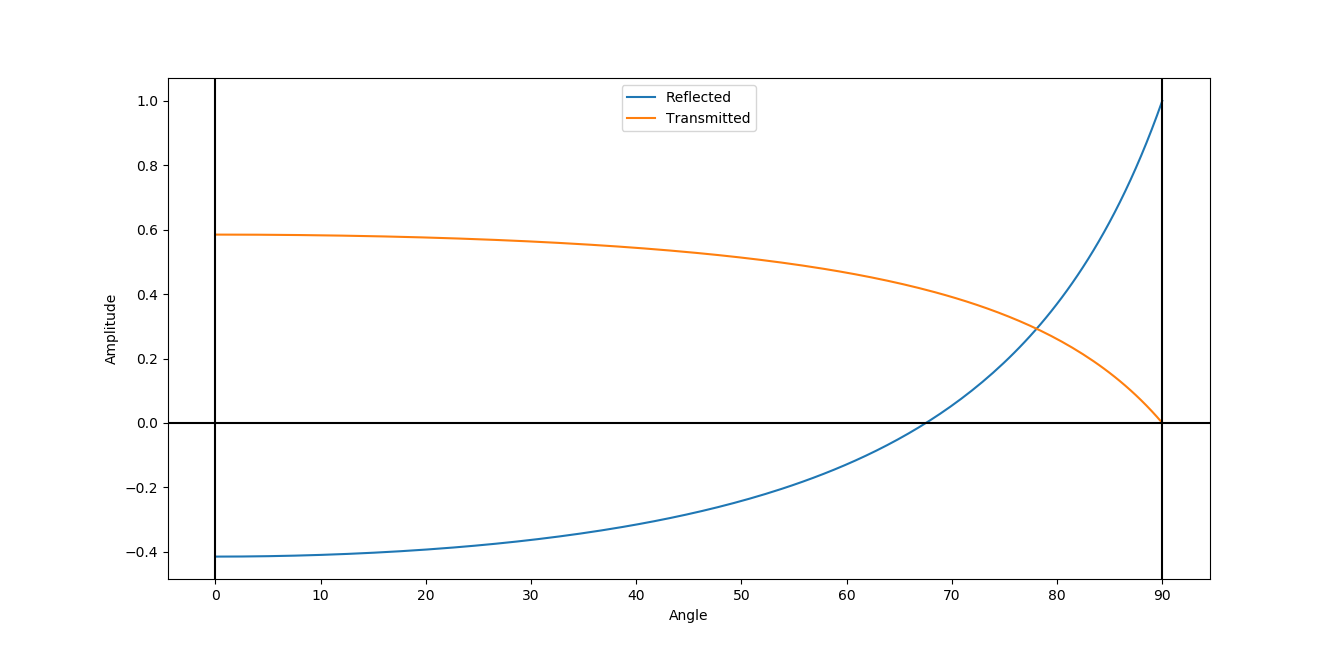
\includegraphics[width=20cm]{graph-9-18.png}}
	\end{center}

	\subsection{Part (a)}

	At normal incidence, $\theta_I = 0$ so
	\begin{align*}
		\alpha &= \frac { \sqrt{ 1 - \beta^2 \sin^2 \theta_I } } { \cos \theta_I
		}\tag{9.110}\\
		&= \frac { \sqrt {1 - \beta^2 (0) } } { (1) }\\
		&= 1\\
	\end{align*}
	Plugging $\alpha$ and $\beta$ into Eq (9.109) yields
	\begin{align*}
		\tilde E_{0_R} &= \frac {\alpha - \beta} {\alpha + \beta} \tilde E_{0_I}
		\tag{9.109}\\
		&= \frac {1 - 2.42} {1 + 2.42} \tilde E_{0_I}\\
		&\approx -0.415 \tilde E_{0_I}\\
		\tilde E_{0_T} &= \frac 2 {\alpha + \beta} \tilde E_{0_I}\tag{9.109}\\
		&= \frac 2 {1 + 2.42} \tilde E_{0_I}\\
		&\approx 0.585 \tilde E_{0_I}
	\end{align*}

	\subsection{Part (b)}

	From Eq. (9.111):
	\begin{align*}
		\sin^2 \theta_B &= \frac {1 - \beta^2} { (n_1/n_2)^2 - \beta^2
		}\tag{9.111}\\
		\theta_B &\approx \arcsin \left( \sqrt { \frac {1 - 2.42^2} {
		(1/2.42)^2 - 2.42^2 } } \right)\\
		&\approx 67.55^\circ
	\end{align*}
	We also could have used Eq. (9.112) as the only requirement to use it over
	(9.111) is $\mu_1 \approx \mu_2$.
	\begin{align*}
		\tan \theta_B &\approx \frac {n_2} {n_1}\\
		\theta_B &\approx \arctan(2.42)\\
		&\approx 67.55^\circ
	\end{align*}

	\subsection{Part (c)}

	\begin{align*}
		\tilde E_{0_R} &= \tilde E_{0_T}\\
		\left( \frac { \alpha - \beta } { \alpha + \beta } \right) \tilde
		E_{0_I} &= \left( \frac 2 { \alpha + \beta } \right) \tilde E_{0_I}\\
		\alpha - \beta &= 2\\
		\alpha &= \beta + 2\\
		&\approx 4.42
	\end{align*}
	Using the definition of $\alpha$, we find
	\begin{align*}
		\alpha^2 &= \frac {1 - \left( \sin^2 \theta \right) / \beta^2 } { \cos^2
		\theta }\\
		1 &= \alpha^2 \cos^2 \theta + \frac {\sin^2 \theta} {\beta^2}\\
		&= \left( \alpha^2 - \frac 1 {\beta^2} \right) \cos^2 \theta + \frac 1
		{\beta^2}\\
		\cos^2 \theta &= \frac {1 - \frac 1 {\beta^2}} {\alpha^2 - \frac 1
		{\beta^2}}\\
		\theta &= \arccos \left( \sqrt { \frac {1 - \frac 1 {\beta^2}} {\alpha^2
		- \frac 1 {\beta^2}} } \right)\\
		&\approx \arccos \left( \sqrt { \frac {1 - \frac 1 {2.42^2}} {4.42^2 -
		\frac 1 {2.42^2}} } \right)\\
		&\approx 78.16^\circ
	\end{align*}

\end{homeworkProblem}

\begin{homeworkProblem}{9.19}
	\renewcommand{\theenumi}{\alph{enumi}}
	\renewcommand{\labelenumi}{(\theenumi)}
	\begin{enumerate}
		\item Suppose you embedded some free charge in a piece of glass. About
		how long would it take for the charge to flow to the surface?
		\item Silver is an excellent conductor, but it's expensive. Suppose you
		were designing a microwave experiment to operate at a frequency of
		$10^{10}$ Hz. How thick would you make the silver coatings?
		\item Find the wavelength and propagation speed in copper for radio
		waves at 1 MHz. Compare the corresponding values in air (or vacuum).
	\end{enumerate}

	\solution

	\subsection{Part (a)}

	From Eq.
	(9.120), the characteristic time for any initial free charge to dissipate is
	\[
		\tau = \frac \varepsilon \sigma
	\]

	Using Wikipedia's table of relative permittivity of some materials at room
	temperature in the article "Relative Permittivity" as source means that
	glass (specifically Pyrex) has a relative permittivity of 4.7. Glass also
	has a resistivity of $10^9$ -- $10^14\Omega$, which means
	\begin{align*}
		\tau &\approx \left( 10^9 \si{\Omega m} \right) (4.7) \left( 8.85 \times
		10^{-12} \si{F/m} \right)\\
		&\approx 0.0416 \si{s}
	\end{align*}
	at the lower bound, but it can get up to around 4000 s if the glass is at
	the high end of the spectrum.

	\subsection{Part (b)}

	We would want the thickness to be above the skin depth, whose definition is
	given by (9.128)
	\begin{align*}
		d &= \frac 1 \kappa\\
		&= \sqrt{ \frac 2 { \omega^2 \varepsilon \mu }} \left( \sqrt{1 + \left(
		\frac \sigma {\varepsilon \omega} \right)^2 } - 1 \right)^{-1/2}\\
		&\approx \sqrt{ \frac 2 { \omega^2 \varepsilon_0 \mu_0 }} \left( \sqrt{1 +
		\left( \frac \sigma {\varepsilon_0 \omega} \right)^2 } - 1
		\right)^{-1/2}\\
		&\approx \sqrt{2} \frac c {2 \pi f} \left( \sqrt{ 1 + \left( \frac
		\sigma {2 \pi \varepsilon_0 f} \right)^2 } + 1 \right)^{-1/2}\\
		&\approx \frac 1 {\sqrt 2} \frac {3 \times 10^8 \si{m/ \cancel s}} {\pi
		10^{10} \si{Hz} } \left( \sqrt{1 + \left( \frac {6.30 \times 10^7
		\si{\Omega m}^{-1} } {2 \pi (8.85 \times 10^{-12} \si{F/m}) (10^{10}
		\si{Hz}) } \right)^2 } - 1 \right)^{-1/2}\\
		&\approx 6.344 \times 10^{-7} \si{m}
	\end{align*}

	\subsection{Part (c)}
	\begin{align*}
		\lambda &= \frac {2 \pi} k\\
		&= 2 \pi \sqrt{ \frac 2 { \omega^2 \varepsilon \mu }} \left( \sqrt{1 +
		\left( \frac \sigma {\varepsilon \omega} \right)^2 } + 1
		\right)^{-1/2}\\
		&\approx 2 \pi \sqrt{ \frac 2 { \omega^2 \varepsilon_0 \mu_0 }} \left(
		\sqrt{1 + \left( \frac \sigma {\varepsilon_0 \omega} \right)^2 } + 1
		\right)^{-1/2}\\
		&\approx \frac {2 \pi c \sqrt 2} \omega \left( \sqrt{1 + \left( \frac
		\sigma {\varepsilon_0 \omega} \right)^2 } + 1 \right)^{-1/2}\\
		&\approx \frac {c \sqrt 2} f \left( \sqrt{1 + \left( \frac \sigma {2 \pi
		\varepsilon_0 f} \right)^2 } + 1 \right)^{-1/2}\\
		&\approx \frac {3 \times 10^8 \sqrt{2}} {10^6 \si{Hz}} \left( \sqrt{ 1 +
		\left( \frac {5.96 \times 10^7 (\si{\Omega m})^{-1}} {2 \pi (8.85 \times
		10^{-12} \si{F/m}) (10^6 \si{Hz})} \right)^2 } + 1 \right)^{-1/2}\\
		&\approx 4.100 \times 10^{-4} \si{m}
	\end{align*}
	which means the speed is
	\begin{align*}
		v &= \lambda f\\
		&\approx (4.100 \times 10^{-4} \si{m}) (10^6 \si{Hz})\\
		&\approx 410.0 \si{m/s}
	\end{align*}
	Both values are orders of magnitude smaller than they would be in a vacuum.

\end{homeworkProblem}

\begin{homeworkProblem}{9.22}
	Calculate the reflection coefficient for light at an air-to-silver interface
	($\mu_1 = \mu_2 = \mu_0, \epsilon_1 = \epsilon_0, \sigma = 6 \times 10^7
	(\Omega \cdot \si{m})^{-1}$), at optical frequencies ($\omega = 4 \times
	10^{15} \si{s^{-1}}$).\\

	\solution

	Using Eq. (9.146) yields
	\begin{align*}
		\tilde \beta &= \frac {\mu_1 v_1} {\mu_2 \omega} \tilde k_2 \\
		&= \frac c \omega (k + i \kappa)
	\end{align*}
	where (from Eq. (9.126))
	\begin{align*}
		k &= \omega \sqrt{ \frac {\varepsilon \mu} 2 } \left( \sqrt{1 + \left(
		\frac \sigma {\varepsilon \omega} \right)^2 } + 1 \right)^{1/2}\\
		\kappa &= \omega \sqrt{ \frac {\varepsilon \mu} 2 } \left( \sqrt{1 +
		\left( \frac \sigma {\varepsilon \omega} \right)^2 } - 1 \right)^{1/2}
	\end{align*}
	Using Eq. (9.115) with a $\theta_I = 0 \implies \alpha = 1$ yields
	\begin{align*}
		R &= \left| \frac {1 - \tilde \beta} {1 + \tilde \beta} \right|^2\\
		&= \frac { \left( 1 - \frac c \omega k \right)^2 + \left( \frac c \omega
		\kappa \right)^2 } { \left( 1 + \frac c \omega k \right)^2 + \left(
		\frac c \omega \kappa \right)^2 }
	\end{align*}
	I originally calculated $\left( \frac c \omega k \right)^2$ because I
	misread my work, but it has cleaner math, so I'm going to keep my
	calculations and then take the square root at the end.
	\begin{align*}
		\left( \frac c \omega k \right)^2 &= \frac {\cancel \omega \cancel {c^2
		\varepsilon \mu}} {2 \cancel \omega} \left( \sqrt {1 + \left( \frac
		\sigma {\varepsilon \omega} \right)^2 } + 1 \right)\\
		&= \frac 12 \left( \sqrt{1 + \left( \frac \sigma { \varepsilon \omega }
		\right)^2 } + 1 \right)\\
		&\approx \frac 12 \left( \sqrt{1 + \left( \frac {6 \times 10^7
		\si{(\Omega \cdot m)}^{-1}} {\left(8.85 \times 10^{-12} \si{F/m} \right)
		\left(4 \times 10^{15} \si{s^{-1}}\right)} \right)^2 } + 1 \right)\\
		&\approx 847.56\\
		\frac c \omega k &\approx 29.11
	\end{align*}
	Calculating $\left( \frac c \omega \kappa \right)^2$ yields
	\begin{align*}
		\left( \frac c \omega \kappa \right)^2 &= \frac {\cancel \omega \cancel
		{c^2 \varepsilon \mu}} {2 \cancel \omega} \left( \sqrt {1 + \left( \frac
		\sigma {\varepsilon \omega} \right)^2 } - 1 \right)\\
		&= \frac 12 \left( \sqrt{1 + \left( \frac \sigma { \varepsilon \omega }
		\right)^2 } - 1 \right)\\
		&\approx \frac 12 \left( \sqrt{1 + \left( \frac {6 \times 10^7
		\si{(\Omega \cdot m)}^{-1}} {\left(8.85 \times 10^{-12} \si{F/m} \right)
		\left(4 \times 10^{15} \si{s^{-1}}\right)} \right)^2 } - 1 \right)\\
		&\approx 846.56
	\end{align*}
	The reflection coefficient is therefore
	\begin{align*}
		R &= \frac { \left( 1 - \frac c \omega k \right)^2 + \left( \frac c \omega
		\kappa \right)^2 } { \left( 1 + \frac c \omega k \right)^2 + \left(
		\frac c \omega \kappa \right)^2 }\\
		&\approx \frac { (1 - 29.11)^2 + 846.56 } { (1 + 29.11)^2 + 846.56 }\\
		&\approx 0.934
	\end{align*}

\end{homeworkProblem}

\end{document}
